%%% -*-LaTeX-*-

\chapter{Bw-Trees}
\label{chap:bw-tree}

We have seen the impact of Zero Copy on network transmission and how that 
compares to the more traditional way of sending data over the network. The difference
in throughput is explicitly seen for smaller 128~B records. Since databases have started
to store all data in memory at all times, database designers have started to normalize 
aggressively and as a result, record sizes are trending smaller and 128~B records show
a more realistic depiction of record sizes in the futures.

At first, the throughput results from comparing Zero Copy and Copy Out for 128~B 
records might tempt  us to think that
it's always better to use a traditional copy. This might be more alluring since we 
 have established that the absolute savings on CPU cycles using Zero Copy may not be 
 significant. 

 One might overlook the bigger problem that lies behind the use of traditional
 copy, that the memory pressure while doing Copy Out occupies a lion share of available
 memory bandwidth. While transmitting at around 7~GB/s(near line rate for the Connect-X3\textregistered),
  we believe the memory pressure will be closer to ~21GB/s which might take up a third of
  all available memory bandwidth in a modern server.

Zero Copy promises memory bandwidth savings in addition to eliminating CPU overhead, 
while Copy Out can saturate the NIC throughput. We wanted to extract the best of both worlds 
and we wanted to analyse structures that can uniquely take advantage of the 
Zero Copy paradigm. 

Microsoft\textregistered Research came up with a modern B-tree structure called 
the Bw-Tree~\cite{bw-tree}, which is a high performance ordered index employing
 lock and latch free concurrency and effective utilisation of caches in 
 modern multi core processors. We discuss it's lock freedom and it's NIC implications
 that make it well suited for Zero Copy in the following sections. We then present
 our evaluation to show the gains in throughput by using delta records in our benchmarks. 

In this chapter, we explore how a client assisted design involving a no-update-in-place 
structure such as Bw-Trees can take advantage of Zero Copy and gain maximum throughput 
without much system impact. We also measure the actual memory bandwidth impact and 
make informed opinions about how these results might apply for designs for other data structures.

\section{Lock-free Indexing}
\label{sec:bwtree-intro}
The Bw-Tree~\cite{bw-tree} is an atomic record store designed for extreme
concurrency. It is an ordered index that supports basic record create, update,
and delete (CRUD) operations in addition to search and range scans.  It is
fully lock-free and non-blocking, and is optimized for modern multicore
workloads. It can store to flash, but is also intended for in-memory
workloads; it serves as the ordered secondary index structure for in-memory SQL
Server Hekaton~\cite{hekaton} engine.

In many ways, the Bw-Tree is a conventional paged B-link tree,
but it also has unique characteristics that interact with network-layer
design choices. Its lock-freedom, its elimination of update-in-place,
and its lazily consolidation of updated records in virtual memory give it
tremendous flexibility in how query results are transmitted by the NIC.

Records may be embedded within leaf pages, or the leaf pages may
only contain pointers to data records. When used as a secondary index,
typically leaf pages would contain pointers, since otherwise each record would
have to be materialized twice and the copies would need to be kept consistent.

\begin{figure}[t]
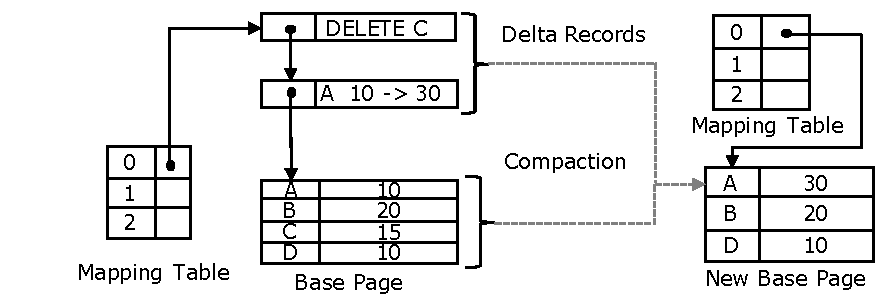
\includegraphics[width=\textwidth]{fig-bwtree.pdf}
\caption{ The structure of a Bw-Tree.}
\label{fig:bw-tree}
\end{figure}

The key challenge in a lock-free structure is providing atomic reads, updates,
inserts, and deletes without ever being able to quiesce ongoing operations (not
even on portions of the tree). Bw-Tree solves this problem by eliminating
update-in-place. All mutations are written to newly allocated memory, then
the changes are installed with a single atomic compare-and-swap instruction
that publishes the change.  Figure~\ref{fig:bw-tree} shows how this works.
A 16KB base page is transmitted here along with a varying number of delta records,
results are shown for both 128~B and 1024~B records.
In place update are avoided by creating delta records ``off to the side'' 
that describe a logical modification to a page. Delta records are
prefixed to a chain ultimately attached to a base page.  When delta chains
grow long they are compacted together with the base page to create a new base page.
All references to pages are translated through a mapping table that maps page
numbers to virtual addresses. This allows pages to be relocated in memory, and
it allows the contents of a page to swapped with a single atomic
compare-and-swap (CAS) operation.

One of the key innovations of the Bw-Tree is its use of {\em delta records},
which make updates inexpensive.
Delta records allow the Bw-Tree to logically modify the
contents of an existing page without blocking concurrent page readers, without
atomicity issues, and without recopying the entire contents of the page for
each update.  Whenever a mutation is made to a page, a small record is
allocated, and the logical operation is recorded within this delta record. The delta
record contains a pointer to the page that it logically modifies. It
is then atomically installed by performing a CAS operation on the
mapping table that re-points the virtual address for a particular page number
to the address of the delta record.

Some threads already reading the original page contents may not see
the update, but all future operations on the Bw-Tree that access that page
will see the delta record. As readers traverse the tree, they consider
the base pages to be logically augmented by their delta records. Delta records
can be chained together up to a configurable length.  When the chain becomes
too long, a new base page is formed that combines the original base page
contents with the updates from the deltas. The new page is swapped-in
the same way as other updates.

Read operations that run concurrent to update operations can observe superseded
pages and delta records, so their garbage collection must be deferred.
To solve this, each thread that
accesses the tree and each unlinked object is associated with a current {\em epoch}.
The global epoch is periodically incremented. Memory for an unlinked object can be
recycled when no thread belongs to its epoch or any earlier epoch.
The epoch mechanism gives operations consistent reads of the
tree, even while concurrent updates are ongoing. However, there is a
cost; if operations take a long time they remain active within their epoch and
prevent reclamation of memory that has been unlinked from the data structure.

\section{NIC Implications for Bw-Tree}

Lock-freedom has major implications on the in-memory layout of the
Bw-Tree. Most importantly, readers (such as the NIC DMA engine) can collect a
consistent view of the tree without interference from writers, and holding that
view consistent cannot stall concurrent readers or writers to the tree.  This
natural record stability fits with the zero-copy capabilities of modern NICs;
because the NIC's DMA engine is oblivious to any locks in the database engine,
structures requiring locking for updates would have to consider the NIC to
have a non-preemtible read lock for the entire memory region until the DMA completes.
Instead of copying records ``out'' of the data structure for transmission,
records can be accessed directly by the NIC. Eliminating the explicit copy of
the records into transmit buffers can save database server CPU and memory
bandwidth.

Page consolidation can also benefit the NIC and improve performance.  Records
in the Bw-Tree are opportunistically packed into contiguous pages in virtual
memory, but the view of a page is often augmented with (potentially many)
small delta
records that are scattered throughout memory.
A database might save CPU and memory bandwidth by more
aggressively deferring or even eliminating consolidation of records into
contiguous regions of memory or pages. We show in
our evalutation that highly discontinuous data can slow
transmission throughput but that aggressive consolidation is inefficient; delta
records can dramatically reduce consolidation overheads while keeping records
sufficiently contiguous to make the NIC more efficient.

Overall, we seek to answer these key questions:
\begin{itemize}
\item
When should records be transmitted directly from a Bw-Tree? Are there cases
where explicitly copying records into a transmit buffer is preferable to gather
DMA operations?
\item
How aggressive should a Bw-Tree be in consolidating records to benefit individual
clients and to minimize database server load?
\item
How does zero-copy impact state reclamation in the Bw-Tree? Might long transmit
times hinder performance by delaying garbage collection of stale records?
\end{itemize}



% Answering these questions?
% - When to tx zero copy versus not?
% - Show tx perf CPU use.


% K: Indexes in modern databases sustain million/op/s.

% K: To support extreme concurrency sometimes lock-free [cite BwTree, ART]

% K: Range scan performance key. But raises key question? How to inexpensively
% get the data to the NIC?

% K: Simplest approach: copy-out results and transmit. Tradtionally this would
% have yielded three copies. One into the results buffer, one for the kernel to
% copy the results into packet buffers, and one for the NIC to DMA the data for
% transmit.

% What about zero-copy? Several problems:
%  - atomicity
%  - garbage collection and object lifetime
%  - packaging the objects for efficient transmit.
%    - pre-package? (paged structures)
%    - use NIC DMA engine?
% Key question? What are the gains?
%  - Reduced copies -> reduced memory bandwidth use, reduced CPU time

% K: Zero-copy? Then data structure must be tied into messaging layer. Can work
% with epoch-based GC, but what about long scans? Could hold back GC and stall
% tree in the limit.




\section{Evaluation}

\subsection{Extending the Delta Format to Clients}

The experiments in the previous chapters consider delivering a clean, ordered set of records to the
client. That is, the server collects and transmits the precise set of records
in the correct order, either via copy-out or zero-copy. Another option is to
transmit base pages along with their deltas and have clients merge the results.
This approach is attractive because it organically fits with the design of the
Bw-Tree and it suits the DMA engine of the NIC well.  The NIC can transmit the
large contiguous base pages (16~KB, for example) with little CPU overhead.
It also eliminates copy-out for small records, but avoids the transmission
throughput ceiling longer gather lists suffer. %(\ref{Chnics-sec:zero-copy-tput}).
Merging records on the client side is cheap; the server can even append them to
the response in a sort order that matches the record order in the base page for
efficient $O(n)$ iteration over the records that requires no copies or sorting.

Figure~\ref{fig:deltas} shows the benefits of this approach. In this
experiment, each transmission consists of a single 16~KB base page while the
number and size of the delta records attached to each transmission is varied.
The NIC benefits from the large base page, and it manages to keep the network
saturated. CPU overhead ranges from less than 1\% when there are a few delta
records up to about 2\% when there are more. Compared to zero-copy of scattered
small records this approach also yields a 1.7$\times$ throughput advantage;
Figure~\ref{fig:zero-copy-tput} shows that throughput peaks at 3.4~GB/s when
records are scattered, while the delta format achieves 5.7~GB/s.
The main cost to this approach is
the cost of consolidating delta records into new base pages when chains grow
long; we consider this overhead in more detail in the next section.

% 3446.988 32 128 B chunks per zero-copy send.
% 5749.283 1 16 KB base page with 4 128 B deltas all zero-copied.
% 5749.283 / 3446.988
% 1.6679150028952816
% = 1.7x

\subsection{Tuning Page Consolidation}
\label{sec:consolidation}


Bw-Tree and many indexing structures are paged in order to amortize storage
access latency, and paging can have similar benefits for network transmission
as well. However, the userlevel access of modern NICs makes interacting with
them much lower-latency than storage devices. This raises the question of
whether paging is still beneficial for in-memory structures. That is, is the
cost of preemptively consolidating updates into pages worth the cost, or is it
better to transmit fine-grained scattered records via zero-copy or copy-out?

%\begin{figure}[H]
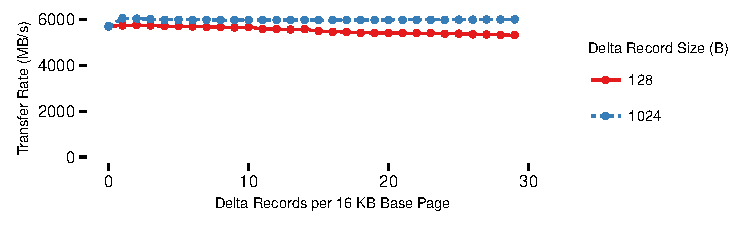
\includegraphics{fig-deltas.pdf}
\caption{Zero Copy transmit performance when transmitting using 
Bw-Tree like delta records}
\label{fig:deltas}
\end{figure}

\begin{figure}[H]
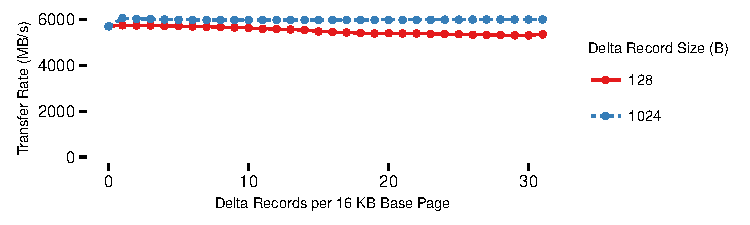
\includegraphics[width=\textwidth]{fig-deltas-tput.pdf}
\caption{Delta Throughput}
\label{fig:deltas-tput}
\end{figure}


\begin{figure}[H]
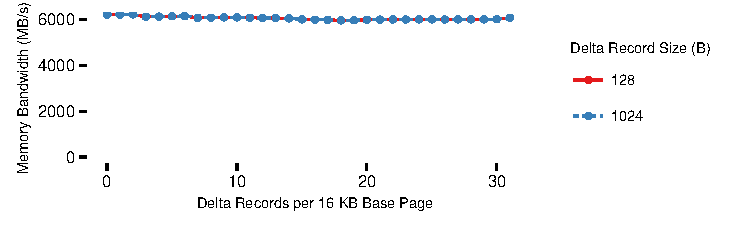
\includegraphics[width=\textwidth]{fig-deltas-membw.pdf}
\caption{Observed Memory Bandwidth Impact varying delta records on a 16~KB base page}
\label{fig:deltas-membw}
\end{figure}



The results of our earlier experiments help answer this question.  If copy-out
is used to gain faster transmission of small records, then the answer is
simple. Even if every update created a complete copy of the full base page, the
extra copies would still be worthwhile so long as more pages are read per
second than updated. This true for most update/lookup workloads, and read-only
range queries make this an even better trade-off.

However, consolidation must be more conservative when using zero-copy to yield
savings, since zero-copy can collect scattered records with less overhead than
copy-out. Yet, there is good reason to be optimistic.  Delta records
reduce the cost of updates for paged structures. If each base page is limited
to $d$ delta records before consolidation, the number of consolidations is
$\frac{1}{d}$. This means that allowing short delta chains dramatically reduces
consolidation costs, while longer chains offer decreasing returns. This fits with
the NIC's preference for short gather lists; allowing delta chains of length 4
would reduce consolidation by 75\% while maintaining transmit throughput that
meets or exceeds on-the-fly copy-out.  The large 16~KB base pages also
improve transmit throughput slightly, which improves efficiency.

For small records, transmitting compacted base pages that have a few deltas gives
a total CPU savings of about 8\%. For the same CPU cost, a server can perform
about 5.2~GB/s of page compaction or about 340,000 compactions per second for
16~KB pages. Even in the worst case scenario where all updates are focused on a
single page, delta chains of length 4 would tolerate 1.3~million updates per
second with CPU overhead lower than copy-out. So, delta records can give the
efficiency of zero-copy with the performance of copy-out.


\subsection{Impact on Garbage Collection}

Using zero-copy tightly couples the higher-level database engine's record
allocation and deallocation, since records submitted must remain stable until
transmission completes. Fortunately, existing mechanisms in systems that avoid
update-in-place accommodate this well, like Bw-Tree's epoch mechanism described
in Section~\ref{sec:bwtree-intro}. Normally, the Bw-Tree copies-out returned records.
While an operation and its copy-out are ongoing, memory that contains records
that have been unlinked or superseded cannot be reclaimed. Zero-copy
effectively defers the copy until the actual time of transmission. As a result,
transmissions completions must notify the higher level database of transmission
completion to allow reclamation. This delay results in more latent garbage and
hurts the effective memory utilization of the system.

In practice, this effect will be small for two reasons. First, zero-copy adds a
transmission, which completes within a few microseconds; however, it also saves a
\memcpy/  which accounts for 1~to~2~$\mu$s for a 16~KB transmission. Second, the
amount of resulting data held solely for transmission should generally be
more than compensated for by eliminating the need for explicit transmit
buffers. With copy-out, the size of the transmit buffer pool is necessarily
larger than the amount of data under active transmission, and internal
fragmentation in the transmit buffers makes this worse.


